\let\negmedspace\undefined
\let\negthickspace\undefined
\documentclass[journal]{IEEEtran}
\usepackage[a5paper, margin=10mm, onecolumn]{geometry}
\usepackage{tfrupee} 

\setlength{\headheight}{1cm}
\setlength{\headsep}{0mm}

\usepackage{gvv-book}
\usepackage{gvv}
\usepackage{cite}
\usepackage{amsmath,amssymb,amsfonts,amsthm}
\usepackage{algorithmic}
\usepackage{graphicx}
\usepackage{textcomp}
\usepackage{xcolor}
\usepackage{txfonts}
\usepackage{listings}
\usepackage{enumitem}
\usepackage{mathtools}
\usepackage{gensymb}
\usepackage{comment}
\usepackage[breaklinks=true]{hyperref}
\usepackage{tkz-euclide} 
\usepackage{listings}

\def\inputGnumericTable{}                                 
\usepackage[latin1]{inputenc}                                
\usepackage{color}                                            
\usepackage{array}                                            
\usepackage{longtable}                                       
\usepackage{calc}                                             
\usepackage{multirow}                                         
\usepackage{hhline}                                           
\usepackage{ifthen}                                           
\usepackage{lscape}

\begin{document}
\bibliographystyle{IEEEtran}
\title{1.4.21}
\author{EE25BTECH11006 - ADUDOTLA SRIVIDYA }
{\let\newpage\relax\maketitle}
\renewcommand{\thefigure}{\theenumi}
\renewcommand{\thetable}{\theenumi}
\setlength{\intextsep}{10pt}
\numberwithin{equation}{enumi}
\numberwithin{figure}{enumi}
\renewcommand{\thetable}{\theenumi}
\parindent 0px

Question:\\
Find the coordinates of the point which divides the line segment joining the points 
$\vec{A}(1,-2,3)$ and $\vec{B}(3,4,-5)$ in the ratio $2:3$ \\
a) internally, and \\
b) externally.\\

\solution\\
Let 
\begin{align*}
    \vec{A} &= \myvec{1\\-2\\3}, \quad 
    \vec{B} = \myvec{3\\4\\-5}
\end{align*}

\textbf{a) Internal Division (2:3)}\\
\begin{align*}
    \vec{P} &= \frac{2\vec{B} + 3\vec{A}}{5} 
             = \myvec{\tfrac{9}{5}\\\tfrac{2}{5}\\-\tfrac{1}{5}}
\end{align*}

\textbf{b) External Division (2:3)}\\
\begin{align*}
    \vec{Q} &= \frac{2\vec{B} - 3\vec{A}}{2-3} 
             = \myvec{-3\\-14\\19}
\end{align*}

\newpage
\begin{figure}[H]
    \centering
    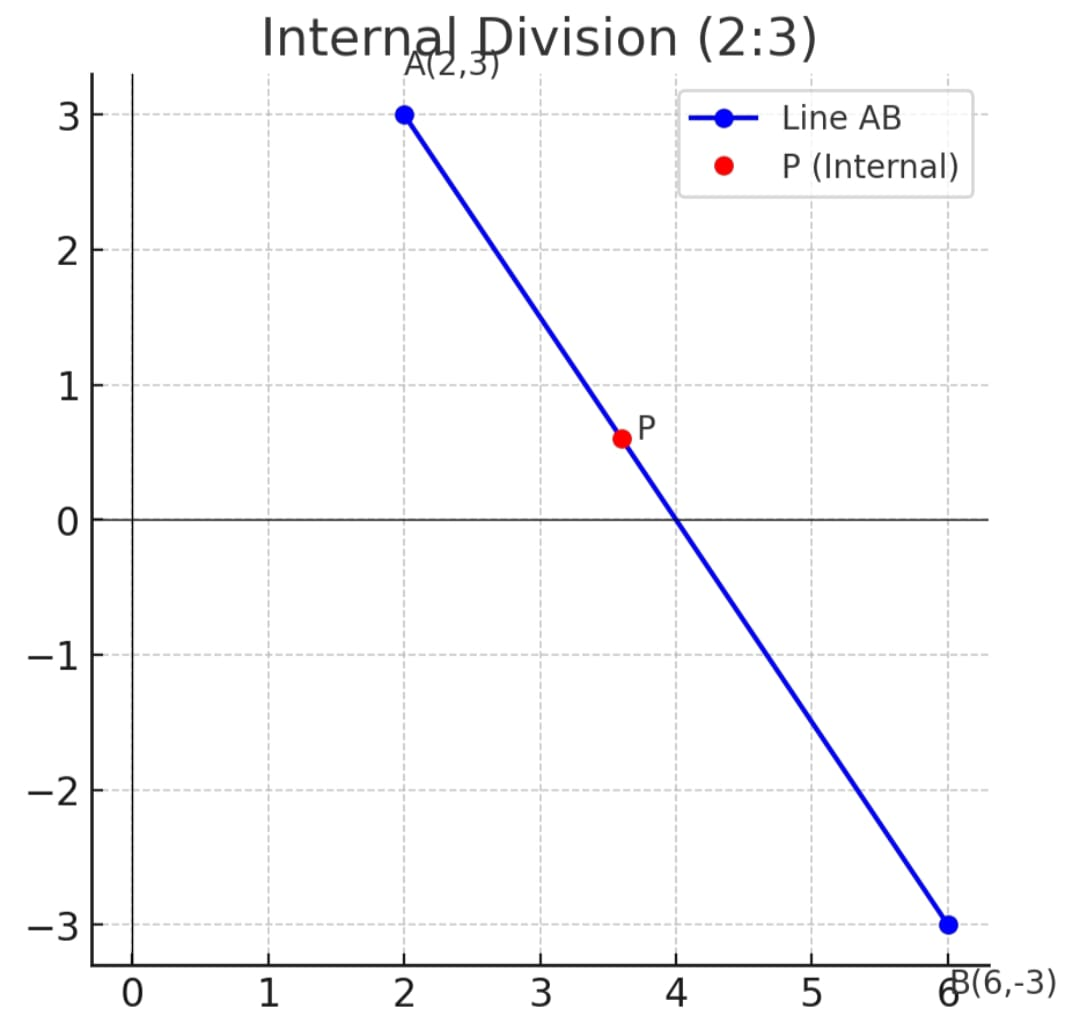
\includegraphics[width=0.5\linewidth]{figs/fig_int_div.jpeg}
    \caption{1}
    \label{fig:1}
\end{figure}
\begin{figure}[H]
    \centering
    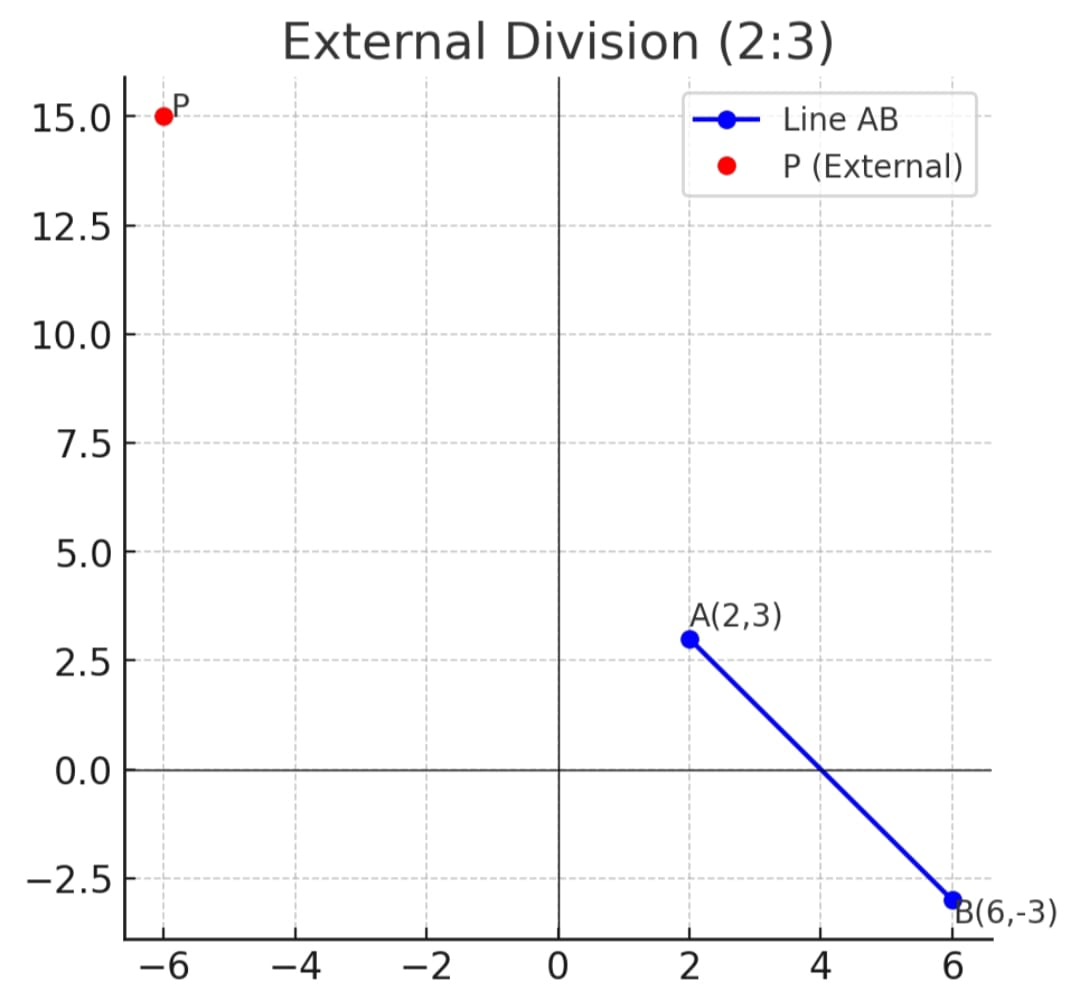
\includegraphics[width=0.5\linewidth]{figs/fig_ext_div.jpeg}
    \caption{2}
    \label{fig:2}
\end{figure}
Therefore, the required points are: \\
Internal: $\brak{\tfrac{9}{5}, \tfrac{2}{5}, -\tfrac{1}{5}}$, \quad 
External: $\brak{-3,-14,19}$.\\



\end{document}